% SC4024 --- Chapter 2: Data Types & Visual Encodings (0->100 ground-up)
\chapter{Data Types \& Visual Encodings}
\label{ch:encodings}
\sloppy

\begin{quote}
\emph{``You cannot encode what you have not understood.''} --- Before choosing a chart, name what kind of thing each column is and what kind of thing the table is. The encoding follows from that naming.
\end{quote}

\noindent\fbox{\parbox{\dimexpr\linewidth-2\fboxsep-2\fboxrule}{%
\textbf{From zero: we build here, no prior data-typing needed.} We assume only tables of values. Every data type, mark, and channel is introduced with intuition before formalism, with small examples and code. No prior visualisation maturity is required.}}
\vspace{0.4em}

\section*{Learning Outcomes}
After this chapter you will be able to:
\begin{enumerate}[label=(L\arabic*)]
    \item classify attributes as nominal, ordinal, quantitative, temporal, and spatial;
    \item distinguish dataset types: tables, networks, fields, geometry, and hierarchies;
    \item define marks (point, line, area) and channels and assign them to data types;
    \item apply expressiveness and effectiveness to critique and fix an encoding;
    \item encode uncertainty and missing data without implying false precision.
\end{enumerate}

% ============================================================
\section{Data Types: WhatKind of Thing Is It?}
\label{sec:data-types}
\paragraph{Intuition.} A column called ``country'' (Singapore, France, Kenya) is not a number---you cannot average it, and sorting it is arbitrary. A column called ``temperature'' is a number where averaging and subtracting mean something. A column called ``shirt size'' (S $<$ M $<$ L) has order but no meaningful subtraction. If you give a nominal column to a channel that implies magnitude, you lie.

\paragraph{Formal view.} Stevens' typology: \emph{nominal} (categories, only $=$ test), \emph{ordinal} (ordered, $<$, no arithmetic), \emph{quantitative} (continuous or discrete, arithmetic meaningful; interval vs ratio depending on whether zero is absolute). Temporal is ordered quantitative with calendrical structure; spatial is inherently 2- or 3-dimensional. Hierarchical or network relations are not attributes but \emph{structures} on items. Keys identify items; values are measured on them.

\begin{definition}[Attribute and dataset types]\label{def:types}
An \emph{attribute} maps items $\to$ values of a type: nominal, ordinal, quantitative (interval/ratio), temporal, spatial. A \emph{dataset type} describes the whole collection: \emph{table} (items $\times$ attributes), \emph{network} (nodes + links + attributes), \emph{field} (continuous domain, e.g.\ temperature over space), \emph{geometry} (shape: points, lines, polygons), \emph{hierarchy/tree}, \emph{cluster/set}.
\end{definition}

\begin{figure}[h]\centering
\begin{tikzpicture}[scale=0.80,every node/.style={font=\scriptsize}]
\node[draw,thick,fill=blue!14,rounded corners=4pt,minimum width=2.6cm,minimum height=1.2cm,align=center] (a) at (0,2.2) {Attributes\\{\tiny nominal/ordinal/quant.}};
\node[draw,thick,fill=green!14,rounded corners=4pt,minimum width=2.6cm,minimum height=1.2cm,align=center] (b) at (4.2,2.2) {Dataset types\\{\tiny table / network / field}};
\node[draw,thick,fill=orange!14,rounded corners=4pt,minimum width=2.6cm,minimum height=1.2cm,align=center] (c) at (8.4,2.2) {Geometry etc.\\{\tiny hierarchy / geometry}};
\draw[->,thick,>=Stealth] (a) -- (b); \draw[->,thick,>=Stealth] (b) -- (c);
% taxonomy tree
\begin{scope}[yshift=-1.2cm]
\node[draw,thick,fill=violet!12,rounded corners=3pt] (root) at (5.4,1.4) {Dataset};
\node[draw,fill=blue!12,rounded corners=3pt] (t1) at (1.2,0) {Tables};
\node[draw,fill=green!12,rounded corners=3pt] (t2) at (3.8,0) {Networks};
\node[draw,fill=orange!14,rounded corners=3pt] (t3) at (6.6,0) {Fields};
\node[draw,fill=yellow!16,rounded corners=3pt] (t4) at (9.2,0) {Geometry};
\draw[thick] (root) -- (t1); \draw[thick] (root) -- (t2); \draw[thick] (root) -- (t3); \draw[thick] (root) -- (t4);
\node[font=\tiny,fill=blue!8,rounded corners=2pt] at (1.2,-0.6) {rows $\times$ cols};
\node[font=\tiny,fill=green!8,rounded corners=2pt] at (3.8,-0.6) {nodes+links};
\node[font=\tiny,fill=orange!8,rounded corners=2pt] at (6.6,-0.6) {grid / continuous};
\node[font=\tiny,fill=yellow!8,rounded corners=2pt] at (9.2,-0.6) {shapes};
\end{scope}
\node[font=\tiny,draw=gray!40,fill=yellow!8,rounded corners=2pt,inner sep=3pt] at (5.4,-1.1) {\textcolor{blue!60!black}{$\blacksquare$ attributes} \quad \textcolor{green!50!black}{$\blacksquare$ datasets} \quad \textcolor{violet!60!black}{$\blacksquare$ hierarchy}};
\end{tikzpicture}
\caption{From attribute types to dataset types. The encoding choice depends on both: a table likes position and bars; a field likes colour and contours; a network likes node-link or matrix.}
\label{fig:datatype-taxonomy}
\end{figure}

Key idea: \emph{keys} vs \emph{values}. A table has independent keys (e.g.\ country, year) and dependent values (e.g.\ GDP). Visual channels for keys should be spatial (position) to show the lookup; values use retinal channels (colour, size, length).

% ============================================================
\section{Marks and Channels}
\label{sec:marks-channels}
\paragraph{Intuition.} Every picture is made of primitive marks: a dot at ($x,y$) for a scatterplot, a line through points for a time series, an area for a bar or polygon. How each mark looks---its position, length, colour, size---encodes data. Position is the richest: it can carry any type precisely. Colour hue is good for categories; saturation and luminance are weaker for numbers.

\begin{definition}[Marks and channels]\label{def:marks}
A \emph{mark} is a geometric primitive: \emph{point} (0-D, dot), \emph{line} (1-D, stroke), \emph{area} (2-D, fill). A \emph{channel} controls a mark's appearance: position ($x,y$), length/height, angle, area, volume, colour hue/saturation/luminance, shape, tilt, texture, motion. Each channel has \emph{type compatibility}: position $\to$ any type; length $\to$ quantitative/ordinal; hue $\to$ nominal; saturation/luminance $\to$ ordinal/quantitative (weak).
\end{definition}

\begin{figure}[h]\centering
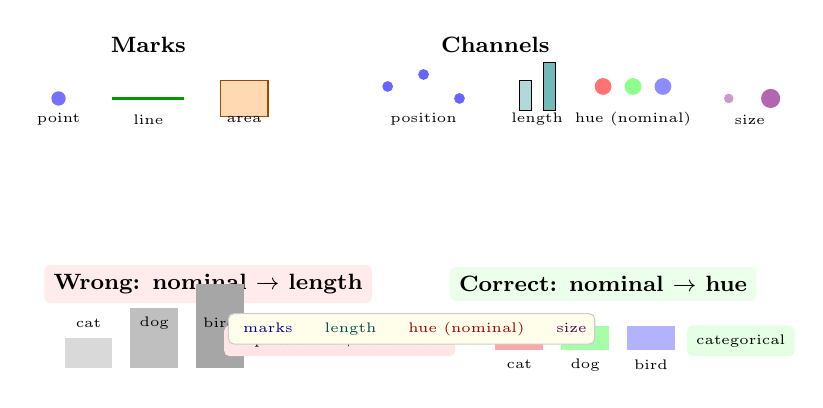
\begin{tikzpicture}[scale=0.76,every node/.style={font=\scriptsize}]
% marks
\node[font=\footnotesize\bfseries] at (2.0,4.2) {Marks};
\fill[blue!55] (0.5,3.3) circle (0.12); \node[font=\tiny] at (0.5,2.95) {point};
\draw[thick,green!60!black] (1.4,3.3) -- (2.6,3.3); \node[font=\tiny] at (2.0,2.95) {line};
\fill[orange!30,draw=orange!60!black] (3.2,3.0) rectangle (4.0,3.6); \node[font=\tiny] at (3.6,2.95) {area};
% channels gallery
\node[font=\footnotesize\bfseries] at (7.8,4.2) {Channels};
% position
\foreach \x/\y in {6/3.5,6.6/3.7,7.2/3.3} \fill[blue!60] (\x,\y) circle (0.09);
\node[font=\tiny] at (6.6,2.95) {position};
% length
\draw[fill=teal!30] (8.2,3.1) rectangle (8.4,3.6); \draw[fill=teal!55] (8.6,3.1) rectangle (8.8,3.9);
\node[font=\tiny] at (8.5,2.95) {length};
% colour hue
\fill[red!55] (9.6,3.5) circle (0.14); \fill[green!45] (10.1,3.5) circle (0.14); \fill[blue!45] (10.6,3.5) circle (0.14);
\node[font=\tiny] at (10.1,2.95) {hue (nominal)};
% size
\fill[violet!40] (11.7,3.3) circle (0.08); \fill[violet!60] (12.4,3.3) circle (0.16);
\node[font=\tiny] at (12.05,2.95) {size};
% expressiveness mismatch demo
\begin{scope}[yshift=-1.6cm]
\node[font=\footnotesize\bfseries,fill=red!8,rounded corners=2pt] at (3.0,1.8) {Wrong: nominal $\to$ length};
\fill[gray!30] (0.6,0.4) rectangle (1.4,0.9); \node[font=\tiny] at (1.0,1.15) {cat};
\fill[gray!50] (1.7,0.4) rectangle (2.5,1.4); \node[font=\tiny] at (2.1,1.15) {dog};
\fill[gray!70] (2.8,0.4) rectangle (3.6,1.8); \node[font=\tiny] at (3.2,1.15) {bird};
\node[font=\tiny,fill=red!10,rounded corners=2pt] at (5.2,0.85) {implies order+ratio: false};
\node[font=\footnotesize\bfseries,fill=green!8,rounded corners=2pt] at (9.6,1.8) {Correct: nominal $\to$ hue};
\fill[red!35] (7.8,0.7) rectangle (8.6,1.1); \node[font=\tiny] at (8.2,0.45) {cat};
\fill[green!35] (8.9,0.7) rectangle (9.7,1.1); \node[font=\tiny] at (9.3,0.45) {dog};
\fill[blue!30] (10.0,0.7) rectangle (10.8,1.1); \node[font=\tiny] at (10.4,0.45) {bird};
\node[font=\tiny,fill=green!10,rounded corners=2pt] at (11.9,0.85) {categorical};
\end{scope}
\node[font=\tiny,draw=gray!40,fill=yellow!8,rounded corners=2pt,inner sep=3pt] at (6.4,-0.55) {\textcolor{blue!60!black}{$\blacksquare$ marks} \quad \textcolor{teal!60!black}{$\blacksquare$ length} \quad \textcolor{red!60!black}{$\blacksquare$ hue (nominal)} \quad \textcolor{violet!60!black}{$\blacksquare$ size}};
\end{tikzpicture}
\caption{Marks (point, line, area) and channels (position, length, hue, size). Bottom: expressiveness mismatch---length implies order and magnitude, so it is wrong for nominal data; hue is correct.}
\label{fig:marks-channels}
\end{figure}

\paragraph{Scales and mappings.} An attribute domain (e.g.\ temperature $[-20,40]$) maps via a \emph{scale} to a channel range (e.g.\ luminance $[10\%,90\%]$ or position $[0,\text{width}]$). Scales may be linear, logarithmic, or custom. Reversed or truncated scales can lie; nominal attributes need categorical (non-ordered) palettes. Always expose the scale: a missing legend turns a picture into a riddle.

% ============================================================
\section{Expressiveness, Effectiveness, and Uncertainty}
\label{sec:express-effective}
Two tests decide a mapping. \emph{Expressiveness}: does the channel say only truths about the data type? (Hue says ``different'' but not ``bigger''---good for nominal, bad for quantitative.) \emph{Effectiveness}: how accurately do eyes read it? (Position $>$ length $>$ angle $>$ area $>$ colour for quantity.)

\begin{example}[Fixing a mismatch]\label{ex:mismatch}
A bar chart that colours countries by GDP uses nominal hue for a quantitative attribute---inexpressive? Actually quantifying colour's luminance is weak; better to use bar length or position. Conversely, mapping ``continent'' to bar length would claim Europe $>$ Asia, which is nonsense. Fix: swap channels so quantitative $\to$ length/position, nominal $\to$ hue.
\end{example}

Uncertainty needs its own channel. \emph{Value-suppressing} palettes fade colour as uncertainty rises; error bars and bands attach to quantitative position encodings. Missing data should not be interpolated silently: show a gap, a hatched mark, or an explicit ``no data'' glyph, otherwise the eye assumes zero.

\begin{figure}[h]\centering
\begin{tikzpicture}[scale=0.78,every node/.style={font=\scriptsize}]
\node[font=\footnotesize\bfseries] at (3.0,3.2) {Uncertainty: value-suppressing};
\foreach \i in {0,...,5} {
  \pgfmathsetmacro{\sat}{90-13*\i}
  \pgfmathsetmacro{\x}{0.55*\i}
  \fill[blue!\sat] (\x,2.0) rectangle +(0.45,0.6);
}
\node[font=\tiny] at (1.6,1.65) {certain $\to$ vivid};
\node[font=\tiny] at (1.6,1.35) {uncertain $\to$ grey};
\node[font=\footnotesize\bfseries] at (7.8,3.2) {Missing data};
\fill[gray!14,draw=gray!40] (6.2,1.9) rectangle (9.4,2.7);
\draw[thick] (6.5,2.0) -- (7.2,2.5) -- (7.9,2.1) -- (8.6,2.6);
\draw[thick,dashed,red!60!black] (7.9,2.1) -- (8.0,2.1) node[midway,below,font=\tiny,fill=red!8,rounded corners=1pt] {gap};
\fill[orange!28,pattern=north east lines,pattern color=orange!60!black] (8.6,1.9) rectangle (9.2,2.7);
\node[font=\tiny,fill=orange!10,rounded corners=2pt] at (8.9,1.65) {hatched = missing};
\node[font=\tiny,draw=gray!40,fill=yellow!8,rounded corners=2pt,inner sep=3pt] at (4.8,0.75) {\textcolor{blue!60!black}{$\blacksquare$ certain} \quad \textcolor{gray!60!black}{$\blacksquare$ uncertain} \quad \textcolor{red!60!black}{$\blacksquare$ gap} \quad \textcolor{orange!60!black}{$\blacksquare$ no data}};
\end{tikzpicture}
\caption{Encoding uncertainty: value-suppressing palettes fade with uncertainty (left); missing data is shown as a gap or hatched region (right), not as zero.}
\label{fig:uncertainty}
\end{figure}

\begin{lstlisting}[language=Python, caption={Altair encodings: binding data types to channels with scales.}, label={lst:altair-enc}]
import altair as alt, pandas as pd

df = pd.DataFrame({"country":["SG","FR","KE"],"gdp":[90,42,6],
                   "continent":["Asia","Europe","Africa"]})
# quantitative -> position+length (bar), nominal -> hue
chart = alt.Chart(df).mark_bar().encode(
    x=alt.X("gdp:Q", scale=alt.Scale(zero=True), title="GDP (quant.)"),
    y=alt.Y("country:N", sort="-x"),
    color=alt.Color("continent:N", legend=alt.Legend(title="Nominal"))
).properties(title="Expressive: Q->length, N->hue")
chart  # in a notebook this renders; .to_json() gives Vega-Lite
\end{lstlisting}

\begin{lstlisting}[language=Python, caption={Value-suppressing sketch and missing-data gaps with Matplotlib.}, label={lst:uncertainty-code}]
import numpy as np, matplotlib.pyplot as plt

x = np.linspace(0, 10, 50)
y = np.sin(x)
uncert = np.linspace(0, 1, 50)          # 0=certain, 1=uncertain
# value-suppressing: alpha fades with uncertainty
plt.figure(figsize=(6,2.5))
for i in range(len(x)-1):
    a = 1 - 0.85*uncert[i]              # fade
    plt.plot(x[i:i+2], y[i:i+2], color="steelblue", alpha=a, lw=2.5)
plt.title("Value-suppressing: certainty -> opacity"); plt.tight_layout()
plt.savefig("suppress.pdf")

# missing data: break the line
y2 = y.copy(); y2[20:28] = np.nan        # gap = missing
plt.figure(); plt.plot(x, y2, color="orange"); plt.title("Gap = missing")
plt.savefig("missing.pdf")
\end{lstlisting}

% ============================================================
\section{Composing Encodings}
\label{sec:compose}
Two attributes can share a view by \emph{composition}: superimposed on the same marks (colour + position), juxtaposed in small multiples, or layered with transparency. Small multiples keep each encoding simple and let position do the heavy lifting; superposition saves space but risks overplotting, rescued by opacity or aggregation. The choice is again an expressiveness trade-off: does the composition imply a false relationship?

% ============================================================
\section{Chapter Notes}
% Notes on typology and encodings
Stevens (1946) typed scales; Bertin (1967) catalogued marks and channels; Mackinlay (1986) formalised expressiveness/effectiveness as automatic design criteria; Munzner (2014) unified attribute and dataset taxonomies; Correll (2018) systematised uncertainty encodings. The next chapter turns ``what to encode'' into ``how to design it well'' via colour and composition.

% ============================================================
\section{Exercises}
\label{sec:ch02-exercises}
\begin{enumerate}[label=E2.\arabic*, leftmargin=*, itemsep=0.8em]
    \item \textbf{Classify.} For the dataset \{student ID, final grade (A--F), essay score 0--100, submission date\}, label each attribute nominal/ordinal/quantitative/temporal and justify. Propose one expressive channel per attribute.
    \item \textbf{Channel critique.} A pie chart shows GDP of 8 countries as slice angles. Using Mackinlay/Cleveland--McGill, argue why a sorted bar chart (length + position) would be more effective for ``which is larger by how much?'' Sketch both and annotate the channel swap.
    \item \textbf{Expressiveness fix.} A designer maps ``blood group (A/B/AB/O)'' to bar length and ``haemoglobin (g/dL)'' to hue. Explain both mismatches and redesign the two encodings so each channel matches its data type.
    \item \textbf{Uncertainty.} You have temperature estimates with 95\% intervals. Design two alternatives: (a) error bars on a line chart, (b) value-suppressing band. When does each fail, and how would you show a sensor outage (missing run)?
    \item \textbf{Altair build.} Using Altair, encode a table with one nominal, one ordinal (shirt size S$<$M$<$L$<$XL), and one quantitative attribute in a single chart without mismatch. Include a Vega-Lite JSON scale that maps ordinal to ordered colour luminance and explain why a rainbow hue would be wrong.
\end{enumerate}
% End of Chapter 2
